%\documentclass[12pt,a4paper]{amsart}
%\usepackage[spanish]{babel}
%\usepackage[all]{xy}
%\CompileMatrices
%\OnlyOutlines
%\ShowOutlines
%\usepackage{amsmath,amssymb,varioref,enumerate}
%\usepackage{emlines2}
%\usepackage[dvipsone]{graphicx}
%\usepackage{epsfig}
%\usepackage{psfrag}
%\newdir{ >}{{}*!/-5pt/\dir{>}}
%\externaldocument{}
%begin numlast
%\newcommand{\lga}{\longrightarrow}
%\newcommand{\lgaf}{\longleftarrow}
%\newcommand {\sub}{\subset}
%\newtheorem{dummy}{realdumb}[section]
%\newtheorem{theorem}[dummy]{Theorem}
%\newtheorem{lemma}[dummy]{Lemma}
%\newtheorem{corollary}[dummy]{Corollary}
%\newtheorem{proposition}[dummy]{Proposition}
%\newtheorem*{theoremun}{Theorem}
%\newtheorem*{corollaryun}{Corollary}
%\theoremstyle{definition}               %%Change Theoremstyle
%\newtheorem{definition}[dummy]{Definition}
%\newtheorem{conjecture}[dummy]{Conjecture}
%\newtheorem{question}[dummy]{Question}
%\newtheorem{example}[dummy]{Example}
%\newtheorem{nothing}[dummy]{Ejercicio}
%\newtheorem{nothing}{Ejercicio}
%\theoremstyle{remark}
%\newtheorem{remark}[dummy]{Remark}
%\newenvironment{display}{\refstepcounter{dummy} $$}%
%{\leqno{\rm ({\thedummy})} $$} \numberwithin{equation}{dummy}
%\theoremstyle{plain}
%end numlast
%\DeclareMathOperator{\co}{co} \DeclareMathOperator{\Diag}{Diag}
%\DeclareMathOperator{\Ar}{Ar} \DeclareMathOperator{\Hom}{Hom}
%\DeclareMathOperator{\coker}{coker} \DeclareMathOperator{\im}{Im}
%\DeclareMathOperator{\R}{\mathbb R}
%\DeclareMathOperator{\N}{\mathbb N}
%\newcommand{\loc}[2]{{\mathcal#1}^{-1}{\mathcal#2}}
%\newcommand{\cat}[1]{\mathcal#1}
%\newcommand{\scat}[1]{\overset{\sim}{\mathcal#1}}
%\newcommand{\ccat}[2]{{\mathcal #1}^{\wedge #2}}
%\newcommand{\complex}[1]{C({\mathcal#1})}
%\newcommand{\ccomp}[2]{C\left({\mathcal#1}^{\wedge#2}\right)}
%\newcommand{\quot}[2]{\left.{\mathcal#1}\!\right/\negmedspace{\mathcal#2}}
%\newcommand{\cquot}[2]{C\left(\left.{\mathcal#1}\!\right/\negmedspace{\mathcal#2}\right)}
%\newcommand{\ccquot}[3]{C\left(\left.
%{\mathcal#1}^{\wedge#3}\right/\negmedspace{\mathcal#2}^{\wedge#3}\right)}
%\newcommand{\qquot}[3]{{\mathcal#1}^{\wedge#3}\negmedspace
%\left.\right/\negmedspace{\mathcal#2}^{\wedge#3}}
%\title{Geometr\'{\i}a y Topolog\'{\i}a de Superficies 2016/17. Relaci\'on 5.}
%\newcommand{\cat}[1]{\mathcal#1}
\documentclass{article}
\usepackage{amsmath,accents}%
\usepackage{amsfonts}%
\usepackage{amssymb}%
\usepackage{comment}
\usepackage{graphicx}
\usepackage{mathrsfs}
\usepackage[utf8]{inputenc}
\usepackage{amsfonts}
\usepackage{amssymb}
\usepackage{graphicx}
\usepackage{mathrsfs}
\usepackage{setspace}
\usepackage{amsthm}
\usepackage{nccmath}
\usepackage[spanish]{babel}
\usepackage{multirow}
\usepackage{hyperref}
\usepackage{tikz-cd}
\usepackage{pgf,tikz}
\usetikzlibrary{arrows}
\usetikzlibrary{cd}
\usetikzlibrary{babel}
\theoremstyle{plain}
\hypersetup{colorlinks=true,citecolor=red, linkcolor=blue}

\renewcommand{\baselinestretch}{1,4}
\setlength{\oddsidemargin}{0.5in}
\setlength{\evensidemargin}{0.5in}
\setlength{\textwidth}{5.4in}
\setlength{\topmargin}{-0.25in}
\setlength{\headheight}{0.5in}
\setlength{\headsep}{0.6in}
\setlength{\textheight}{8in}
\setlength{\footskip}{0.75in}

\theoremstyle{definition}

\newtheorem{theorem}{Teorema}[section]
\newtheorem{acknowledgement}{Acknowledgement}
\newtheorem{algorithm}{Algorithm}
\newtheorem{axiom}{Axiom}
\newtheorem{case}{Case}
\newtheorem{claim}{Claim}
\newtheorem{propi}[theorem]{Propiedades}
\newtheorem{condition}{Condition}
\newtheorem{conjecture}{Conjecture}
\newtheorem{coro}[theorem]{Corolario}
\newtheorem{criterion}{Criterion}
\newtheorem{defi}[theorem]{Definición}
\newtheorem{example}[theorem]{Ejemplo}
\newtheorem{exercise}{Ejercicio}
\newtheorem{lemma}[theorem]{Lema}
\newtheorem{nota}[theorem]{Nota}
\newtheorem{sol}{Solución}
\newtheorem*{sol*}{Solución}
\newtheorem{prop}[theorem]{Proposición}
\newtheorem{remark}{Remark}

\newtheorem{dem}[theorem]{Demostración}

\newtheorem{summary}{Summary}

\providecommand{\abs}[1]{\lvert#1\rvert}
\providecommand{\norm}[1]{\lVert#1\rVert}
\providecommand{\ninf}[1]{\norm{#1}_\infty}
\providecommand{\numn}[1]{\norm{#1}_1}
\providecommand{\gabs}[1]{\left|{#1}\right|}
\newcommand{\bor}[1]{\mathcal{B}(#1)}
\newcommand{\R}{\mathbb{R}}
\newcommand{\Q}{\mathbb{Q}}
\newcommand{\Z}{\mathbb{Z}}
\newcommand{\F}{\mathbb{F}}
\newcommand{\X}{\chi}
\providecommand{\Zn}[1]{\Z / \Z #1}
\newcommand{\resi}{\varepsilon_L}
\newcommand{\cee}{\mathbb{C}}
\providecommand{\conv}[1]{\overset{#1}{\longrightarrow}}
\providecommand{\gene}[1]{\langle{#1}\rangle}
\providecommand{\convcs}{\xrightarrow{CS}}
% xrightarrow{d}[d]
\setcounter{exercise}{0}
\newcommand{\cicl}{\mathcal{C}}
\begin{document}

\title{Relación 5 - Geometría y Topología de superficies }
\author{Javi, Rafa, Diego}
\maketitle

%\begin{exercise} \label{E1.2} Si ${B}^{n}$ es la bola eucl\'{\i}dea $n$-dimensional e $Y$
%es  un espacio arcoconexo, probar que toda aplicaci\'on de
%${B}^{n}$ en Y es homot\'opica a la aplicaci\'on constante.
%\end{exercise}
%
%\newpage

\begin{exercise} Probar que al identificar dos puntos de una esfera se obtiene un espacio que no es simplemente conexo.
\end{exercise}
\begin{sol*}Si el grupo fundamental de $X$ fuese trivial y nos fijamos en la circunferencia $S^1$ en trazo grueso tenemos que $X$ se retrae sobre $S^1$ (ver dibujo).
\begin{center}
\begin{figure}[h!]
	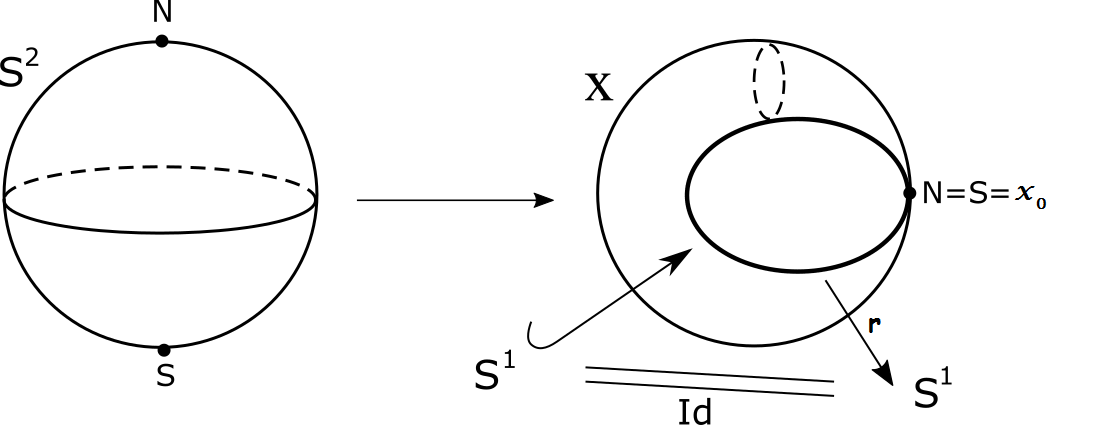
\includegraphics[scale=0.3]{bitmap}
\end{figure}
\end{center}
Tendríamos la composición $S^1\hookrightarrow X\to S^1$ en el que la última composición proyectaría cada sección de circunferencia sobre un punto de $S^1$. Esta última aplicación es continua y los elementos de $S^1$ no se mueven, por lo que se trata de una retracción, luego se induce el siguiente diagrama 
\[
\begin{tikzcd}
\Z\cong\pi_1(S^1,x_0)\arrow[r,"i_* "] \arrow[rr,"(r\circ i)_*=Id_*=Id",bend left=10] &  \pi_1(X,x_0)\cong\{1\}\ar[r, "r_* "] & \pi_1(S^1,x_0)\cong\Z\\
\end{tikzcd}
\]
Ello implicaría que la identidad de $\Z$ sería el homomorfismo nulo, lo que es una contradicción. 
\end{sol*}

\newpage

\begin{exercise} Probar que la circunferencia es un retracto del toro $S^1\times S^1$, pero que no puede ser retracto de deformaci\'on.
\end{exercise}
\begin{sol*}
Para probar que es retracto basta tomar la proyección $p_1:S^1\times S^1\to S^1$. Pero no puede ser retracto de deformación porque los retractos de deformación conservan los grupos fundamentales, sin embargo $\pi_1(S^1\times S^1)=\Z\times\Z\not\cong\Z =\pi_1(S^1)$.
\end{sol*}

\newpage

\begin{exercise} \label{grado1} De acuerdo con el Ejercicio 9 de la relaci\'on 4, por ser $\pi_1(S^1,z_0)$ abeliano, dados dos caminos cualquiera $\gamma$ y  $\gamma'$ entre $z$ y $z_0$, los isomorfismos $\gamma_{\#}$ y $\gamma'_{\#}$ coinciden. Por tanto se tiene un isomorfismo can\'onico $\gamma_{z_0,z}: \pi_1(S^1,z_0) \cong \pi_1(S^1,z)$. Sea $z_0 = 1$ la unidad compleja y $\varepsilon_0 = [\alpha_1]$ es la clase del lazo en $z_0$ $\alpha_1: I \to S^1$ dado por $\alpha_1(t) = e^{2\pi it}$ que, ya sabemos, genera $\pi_1(S^1,z_0)$. Para cada $z\in S^1$, tomamos el generador $\varepsilon_z = \gamma_{z_0,z}(\varepsilon_0)$.
\par
Dada una aplicaci\'on $f: S^1\to S^1$, se llama \emph{grado} de $f$ al entero $grad(f) = n\in \mathbb{Z}$ que cumple $f_*(\varepsilon_0) = n \varepsilon_{f(z_0)}$ siendo $f_*: \pi_1(S^1,z_0) \to \pi_1(S^1,f(z_0))$.
\begin{enumerate}
\item Probar que $grad(f)$ no depende de la clase de homotop\'{\i}a de $f$.
\item Probar $grad(g\circ f) = grad(g) \ grad(f)$.
\item Si $\widetilde{\beta}: I \to \mathbb{R}$ es la elevaci\'on del lazo en $z_0$ $\beta: I \to S^1$, entonces  $grad(\beta)$ es el
entero que cumple $\widetilde{\beta}(1) = 2grad(\beta) \pi$; es decir el grado de $\beta$ tal y como se defini\'o en el tema sobre el c\'alculo del grupo fundamental de $S^1$.
\item Probar que dado $0\leq \theta_0 \leq 2\pi$, la aplicaci\'on (giro de \'angulo $\theta_0$) $g: S^1\to S^1$ dada por $g(z) =  e^{i\theta_0}z$ es homot\'opica a la identidad.
    \item Usar el apartado anterior para probar que el grado de cualquier aplicaci\'on $f: S^1\to S^1$ es igual al del lazo en $z_0$ $e^{i\theta_0}f$ donde $z_0 = e^{i\theta_0} f(z_0)$.
\end{enumerate}
\end{exercise}

\newpage

\begin{exercise}
Sea $f:B^2 \to \mathbb{R}^2$ una aplicaci\'on tal que $f(S^1) \subset S^1$ y
$grad (f|S^1)\neq 0$. Probar que la bola $B^2$ debe estar contenida en la imagen de $f$.
\end{exercise}

\newpage

\begin{exercise}
\item \label{pl11.n1}
Sea $f:S^1\times S^1 \to S^1 \times S^1$ la aplicaci\'on (como n\'umeros complejos) $f(z,w)=(z^a
w^b,z^c w^d)$ con $a,b,c,d \in \mathbb{Z}$. Dar el homomorfismo inducido
$f_*: \pi_1(S^1\times S^1,(z_0,z_0)) \to \pi_1(S^1\times S^1,(z_0,z_0))$, donde $z_0 = 1$ es la unidad compleja.
\end{exercise}

\newpage

\begin{exercise}
Probar que para una aplicaci\'on $f: S^1\to S^1$ se tiene $grad(f) = n$ si y s\'olo si $f\simeq \alpha_n$ sonde
$\alpha_n(z) = z^n$ (en n\'umeros complejos).
\end{exercise}

\newpage

\begin{exercise} Se probar\'a el teorema fundamental del \'algebra: todo polinomio complejo
polinomio complejo $f(z)=a_nz^n + a_{n-1}z^{n-1}+\dots + a_0$
de grado mayor o igual que uno tiene una ra\'{\i}z. Para ello se proceder\'a en los siguientes pasos:
\begin{enumerate}
\item Sin p\'erdida de generalidad podemos considerar que $a_n=1$ y $a_0 \neq 0$.
Suponiendo que $f(z)\neq 0$ para todo $z\in \mathbb{C}$, se toma $M = \max\{1, n|a_{n-1}|, n|a_{n-2}|, \dots ,n|a_0|\}$. Comprobar que si $|z|\ge M$ se tiene $|z^j|\leq |z^{n-1}|$ para $j\leq n-1$, de donde

$$
|a_{n-1}z^{n-1}+\dots + a_0|\le |a_{n-1}| |z^{n-1}|+\dots + |a_0| \le
$$
$$ (|a_{n-1}|+\dots + |a_0|)|z^{n-1}|
\le M |z^{n-1}|\le |z^n|.
$$
\item Consideremos $H:\mathbb{C} \times I \to \mathbb{C}$ definida como
$H(z,t)=z^n+t(a_{n-1}z^{n-1}+\dots + a_0)$. Comprobar que si $|z|\ge M$ entonces
$H(z,t)\ne 0$.
\item Verificar que las homotop\'{\i}as $F, G: S^1\times I \to S^1$ dadas por
$F(z,t)=\frac{f(Mtz)}{|f(Mtz)|}$
y $G(z,t)=\frac{H(Mz,t)}{|H(Mz,t)|}$ est\'an bien definidas.
\item Deducir que la aplicaci\'on $f_n(z)=z^n$ es homot\'opica a la aplicaci\'on constante
$\frac{a_0}{|a_0|}$ y llegar a contradicci\'on.
\end{enumerate}
\end{exercise}
\begin{sol*}
En primer lugar definimos $f_n:S^1\to S^1$ como $f_n(z)=z^n$. Obsérvese que $z^n=e^{2\pi nti}=\cos(2\pi nt)+i\sen(2\pi nt)$. De esta forma, el homomorfismo inducido por $f_n$,
\[
f_{n*}:\pi_1(S^1,(1,0))\to \pi_1(S^1,(1,0))\\
\]
lleva el generador $[\alpha]$ representado por $\alpha(t)=e^{2\pi it}$ en la clase de $\alpha_n(t)=e^{2\pi i nt}$ cuyo grado es $n$. Así que $f_{n*}[\alpha]=[\alpha_n]=n[\alpha]$.\\
Ahora pasamos a razonar por reducción al absurdo. Supongamos que $p(z)\neq 0\ \forall z\in\mathbb{C}$. Podemos suponer que $p(z)$ es mónico, pues en caso contrario bastaría con dividir por el término líder. Es decir, vamos a trabajar con $p(z)=z^n+\cdots + a_0$. Sea $M=\max\{1,|a_{n-1}|+\dots +|a_0|\}$. Si $|z|\geq M$, entonces $|z|^j\leq |z|^{n-1}$ para $j\leq n-1$. Además,
\[
|a_{n-1}z^{n-1}+\cdots +a_0|\leq |a_{n-1}||z|^{n-1}+\cdots +|a_0|\leq (|a_{n-1}|+\dots +|a_0|)|z|^{n-1}\leq M|z|^{n-1}\leq|z|^n.
\]
Definimos ahora las homotopías $F:S^1\times I\to S^1$ y $G:S^1\times I\to S^1$ de la siguiente forma
\[
F(z,t)=\frac{p(Mtz)}{|p(Mtz)|}\quad G(z,t)=\frac{H(z,t)}{|H(z,t)|},
\]
donde $H:\mathbb{C}\times I\to\mathbb{C}$ es la función $H(z,t)=z^n+t(a_{n-1}z^{n-1}+\cdots +a_0)$. Se tiene que $F$ es continua porque suponemos $p(z)\neq 0\ \forall z\in\mathbb{C}$. La continuidad de $G$ es inmediata pues el denominador no se anula nunca. En efecto, al ser $|z|\geq M$
\begin{gather*}
H(z,t)=0\Rightarrow z^n+t(a_{n-1}z^{n-1}+\cdots +a_0)=0\Rightarrow \\
z^n=-t(a_{n-1}z^{n-1}+\cdots +a_0)\Rightarrow |z|^n=t|a_{n-1}z^{n-1}+\cdots +a_0|
\end{gather*}
Pero esto significaría que para $0<t<1$, $|z|^n<|a_{n-1}z^{n-1}+\cdots +a_0|\leq|z|^n$, con lo que hemos llegado a una contradicción. Observemos ahora lo siguiente
\begin{gather*}
F(z,0)=\frac{p(0)}{|p(0)|}=1\ (cte)\qquad F(z,1)=\frac{p(Mz)}{|p(Mz)|}\\
G(z,0)=\frac{z^n}{|z|^n}=z^n=f_n(z)\quad G(z,1)=\frac{p(Mz)}{|p(Mz)|}
\end{gather*}
Por transitividad de la relación de homotopía $cte\simeq f_n(z)$. Este resultado nos conduce, considerando el camino $\gamma(t)=H((1,0),t)$ al siguiente diagrama
\[
\begin{tikzcd}
\pi_1(S^1,(1,0)) \ar[r, "f_{n*} "]\arrow[d,"cte_* "'] & \pi_1(S^1,(1,0))\\
\pi_1(S^1,q)\arrow[ur,"\gamma_\sharp "',"\cong"]
\end{tikzcd}
\]
Pero esto es una contradicción porque $f_{n*}\neq 0$, y $cte_*$ es el homomorfismo trivial. 
\end{sol*}

\newpage

\begin{exercise} \label{grado2} Sea ·$f: S^1\to S^1$ una aplicaci\'on tal que $f(-z) = -f(z)$ para todo $z\in S^1$. Se quiere demostrar que $grad(f)$ es impar.
\begin{enumerate}
\item Probar que si $z_0 = e^{i\theta_0}f(z_0)$, entonces la aplicaci\'on $h = e^{i\theta_0}f(z)$ cumple tambi\'en $h(-z) = -h(z)$. En particular, para el lazo $\alpha_1(t) = e^{2\pi i t}$  se cumple que $h\circ \alpha_1(t+\frac{1}{2}) = -h \circ \alpha_1(t)$ para todo $t\in [0,\frac{1}{2}]$.

\item Comprobar que la elevaci\'on del lazo $h\circ \alpha_1$ por $0\in \mathbb{R}$,
$\widetilde{h\circ \alpha_1}$, cumple, para $t\in [0,\frac{1}{2}]$, $\widetilde{h\circ \alpha_1}(t+\frac{1}{2}) = \widetilde{h\circ \alpha_1}(t) +\frac{q(t)}{2}$, donde $q(t)$ es un entero impar, que, en principio depende de $t$. Probar que $q(t) = q$ para todo $t$.
\item Deducir del apartado anterior que $h_*: \pi_1(S^1,z_0) \to \pi_1(S^1,z_0)$ cumple $h_* ([\alpha_1]) = q [\alpha_1]$. Por tanto, el grado de la aplicaci\'on original $f$ es impar.

\end{enumerate}
\end{exercise}

\newpage

\begin{exercise}
Probar que las siguientes afirmaciones son equivalentes, y que son consecuencias del Ejercicio \ref{grado2} (todas las aplicaciones se suponen continuas).
\begin{enumerate}
\item  En todo recubrimiento de $S^2$ por tres conjuntos cerrados $A_1, A_2, A_3$, existe un $A_i$ que contiene un par de puntos antipodales.
(\emph{Teorema de Lusternik-Schnirelmann-Borsuk}).
\item No existen aplicaciones $f: S^2\to S^1$ que preserven puntos antipodales; esto es, $f(-x) = -f(x)$.
\item Una aplicaci\'on $f: S^1\to S^1$ que preserve puntos antipodales no puede ser homot\'opicamente trivial.
\item Toda aplicaci\'on $f: S^2\to \R^2$ identifica al menos dos puntos
antipodales; es decir, existe $x_0\in S^2$ con $f(x_0) = f(-x_0)$. (Teorema de Borsuk-Ulam).
\end{enumerate}
Para probar  (1) $\Rightarrow$ (2) usar el recubrimiento de $S^1$ por los tres arcos comprendidos entre las ra\'{\i}ces c\'ubicas de la unidad. Para
(4) $\Rightarrow$ (1) usar la aplicaci\'on $f: S^2\to \mathbb{R}^2$ dada por $f(x) = (d(x,A_1), d(x,A_2))$.
\end{exercise}
\begin{sol*}
$\boxed{(1) \Rightarrow (2)}$ Lo probamos por reducción al absurdo. Supongamos que $\exists f:S^1\to S^1$ tal que $f(-x)=-f(x)$. Vamos a considerar el recubrimiento indicado en el enunciado y llamamos a cada arco $B_1$, $B_2$ y $B_3$ respectivamente. Denotamos $A_i=f^{-1}(B_i)\ i=1,2,3$. Si $A_i$ contiene puntos antipodales, entonces $f(A_i)$ también, pero $B_i$ no contiene puntos antipodales, con lo que hemos llegado a contradicción.\\
$\boxed{(2) \Rightarrow (3)}$ Razonamos por reducción al absurdo. Sea $f: S^1\to S^1$ preservando puntos antipodales y supongamos que es homotópicamente trivial. Por un ejercicio de la relación anterior, $f$ se extiende de forma continua a $g:B^2 \to S^1$. Podemos identificar $B^2$ con una semiesfera, de modo que en la otra semiesfera definimos $g'(x)=-g(-x)$. Consideremos $x\in S^1$, entonces
\[ g'(x)=-g(-x)=-f(-x)=f(x).\]
Por lo aplicación $g\cup g' :S^2\to S^1$ preserva puntos antipodales y hemos llegado a una contradicción.\\
$\boxed{(3) \Rightarrow (4)}$ Utilizamos reducción al absurdo. Supongamos que $\exists f:S^2\to\R^2$ que no identifica puntos antipodales. Vamos a ver que existe $g:S^1\to S^1$ que preserva puntos antipodales y es homotópicamente trivial. Consideramos 
\begin{align*}
h&:S^2\to\R^2 & h'&:S^2\longrightarrow S^1\\
 &x\longmapsto f(x)-f(-x) & &x\longmapsto\frac{f(x)-f(-x)}{||f(x)-f(-x)||}
\end{align*}
que está bien definida porque $f$ no identifica puntos antipodales. Entonces podemos considerar
\[
\begin{tikzcd}
S^1\arrow[r,"i",hookrightarrow]\arrow[rr,"g"', bend right=20]& S^2\arrow[r,"h'"]& S^1
\end{tikzcd}
\]
Se tiene que $g$ preserva antipodales y además es homotópicamente trivial, pues $h$ es homotópicamente trivial y podemos usarla para encontrar una composición $$S^1\to S^2\to\R^2\to S^1.$$
$\boxed{(4) \Rightarrow (1)}$ Vamos a probar que $\{(4),\neg (1)\}\models \perp$. Supongamos que ninguno de los tres cerrados contiene puntos antipodales. Usamos la aplicación del enunciado $f: S^2\to \mathbb{R}^2$ dada por $f(x) = (d(x,A_1), d(x,A_2))$. Por hipótesis existe $x_0\in S^2$ tal que $f(x_0)=f(-x_0)$. Supongamos que $x_0\in A_3$. Entonces $-x_0\notin A_3$, por tanto $-x_0\in A_1\cup A_2$. De modo que $d(x_0,A_1)$ y $d(x_0,A_2)$ son estrictamente positivas, pero o bien $d(-x_0,A_1)=0$ o bien $d(-x_0,A_2)=0$, contradiciendo que $f(x_0)=f(-x_0)$. Si $x_0$ pertenece a otro cerrado se razona de forma análoga.
\end{sol*}

\newpage

\begin{exercise}
Sean $A_1$ y $A_2$ dos conjuntos medibles y acotados de $\mathbb{R}^2$. Probar que existe una recta en el plano que parte a $A_1$ y $A_2$ en conjuntos de la misma medida. Para ello considerar $\mathbb{R}^2= \mathbb{R}^2\times
\{1\}\subseteq \mathbb{R}^3$  y para cada vector unitario $x\in \R^3$
se toman $V_x= \mathbb{R}^2\times \{1\} \cap \{y\in \R^3;\; x.y\ge 0\}$
y $H_x= \{y\in V_x;\; x.y = 0\}$. Aqu\'{\i} $x.y$ denota el producto escalar.
Entonces definir  $f = (f_1, f_2): S^2 \to \R^2$ por $f_i(x)= m(A_i\cap
V_x)$, la medida de  $A_i\cap V_x$. Aplicar a $f$ el teorema de Borsuk--Ulam.
\end{exercise}

\newpage

\begin{exercise}
Sea $X$ un espacio conexo por caminos tal que $\pi_1(X,x_0)$ no contiene un subgrupo isomorfo a $\mathbb{Z}$. Supongamos que existen aplicaciones
$f: X\to X$ y $g: S^1 \to X$ tales que
$fg(z) = g(-z)$ y $f^2=Id$. Probar que para cualquier aplicaci\'on  $h: X\to \mathbb{R}^2$ existe $x\in X$ tal que $h(x) = hf(x)$. Para ello suponer lo contrario y considerar  el grado de la composici\'on $\widetilde{h} g: S^1
\rightarrow S^1$ donde $\widetilde{h}(x) =
h(x)-hf(x)/\|h(x)-hf(x)\|$.
\end{exercise}

\newpage

\begin{exercise} Probar que toda matriz cuadrada
$A= (a_{ij})_{1\le i,j\le 3}$ con $a_{ij}> 0$ para todo $i,j$, tiene al menos un
autovalor positivo
(\emph{Teorema de Perron--Frobenius}). Para ello aplicar el teorema del punto fijo de
Brouwer a la aplicaci\'on $g: \Delta^2\to \Delta^2$ dada por $g(x)= Ax/\sigma(Ax)$ donde $\Delta^2\subset \R^3$ es el tri\'angulo de
v\'ertices los puntos $(1,0,0)$, $(0,1,0)$ y $(0,0,1)$ y  $\sigma: \R^3\to \R$ es la suma de coordenadas.
\end{exercise}

\newpage

\begin{exercise}
Sea $f:\R^2\to \R^2$ una aplicaci\'on con $f^2= id$ (y por tanto homeomorfismo). Probar que $f$ tiene un punto fijo. Para ello sean $S^0 \subseteq S^1 \subseteq S^2$ las inclusiones de los correspondientes ecuadores y construir aplicaciones $g_0: S^0 \to \R^2$, $g_1: S^1\to \mathbb{R}^2$ y $g_2: S^2\to \mathbb{R}^2$ con $g_1=g_0$ en $S^0$ y $g_2 = g_1$ en $S^1$, cumpliendo $g_k(-x) = f(g_k(x))$. Entonces aplicar el teorema de Borsuk a $g_2$.
\end{exercise}




\end{document}
